\scanpage{79}

% heading
$(\unsure{\mathrm I|+})$ Étude combinatoire des polygones de $3\le n\le6$ côtés

% upper left, sideways note
% margin note written sideways
\margin{On obtient les sous-groupes comme stabilisateurs des sommets (ou côtés) et $\unsure{\sim}$ \unsure{d'un|chacun|chaque} élt de $\unsure{\omega}(T)$\deleted{\illegible{1}}}

% top, 1), lines 2–5
1) \uline{$n=3$}\quad $\mathrm{Pol}_3\simeq(\mathrm{Ens})_3$, le foncteur de dualité est isom can à l'identité (si $P\in\mathrm{Ob}\,\mathrm{Pol}_3$, alors $P^\circ\simeq P$ (iso can.) car les côtés en corr $1-1$ avec les sommets. (Se généralise aux polygônes à un nb impair de côtés. Groupe : $\mathfrak S_{3}$

% upper, 2), lines 6–8
2) \uline{$n=4$}\quad $\mathrm{Pol}_4\xrightarrow{\sim}(\mathrm{Ens})_{2,2}$ (se généralise aux cubes comb. de dim $d\in\mathbb N$, $\mathrm{Cube}_d\simeq(\mathrm{Ens})_{\underbrace{2,2,\ldots,2}_{d}}$) Obtenu en associant à \deleted{\unsure{un C}} carré comb. $C$ l'ens de ses quatre côtés, avec la division en côtés opposés.

% middle, lines 9–15
Le cube combinatoire dim. $2$ est décrit par l'ens des $4$ sommets, avec division en classes de sommets \deleted{\unsure{opposables|opposés}}. Or les sommets correspondent aux sections de $I$ sur $\Lambda$, l'incidence signifiant que les \deleted{côtés} sections ne se rencontrent pas, l'opposition $=$ non incidence signifiant qu'ils sont ``parallèles'' --

% middle left, beside description
\figure{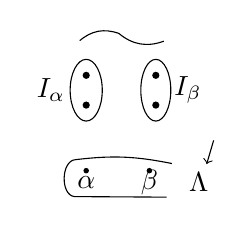
\begin{tikzpicture}[x=.68cm,y=.7cm]
\draw (0,1.1) ellipse (.3 and .56) (1.3,1.1) ellipse (.28 and .56);
\foreach \x in {0,1.3}{\foreach \y in {.83,1.37}{\fill (\x,\y) circle (1.3pt);}}
\node at (-.66,1.1) {$I_\alpha$};\node at (1.9,1.1) {$I_\beta$};
\draw (-.12,2) to[bend left] (.61,2.13) to[bend right] (1.45,1.99);
\draw (1.6,-.23) to[bend right=9] (-.2,-.16) to[bend right=85] (-.22,-.83)--(1.5,-.84);
\node at (0,-.58) {$\alpha$};\node at (1.18,-.58) {$\beta$};\fill (0,-.36) circle (1pt) (1.18,-.36) circle (1pt);
\node at (2.1,-.56) {$\Lambda$};\draw[->] (2.38,.19)--(2.25,-.24);
\end{tikzpicture}}

% lower left, cubical diagram
\diagram{\begin{tikzcd}[ampersand replacement=\&,cells={font=\small},row sep=1.3em,column sep=1.4em]
\& C_s\arrow[dl,"2" description,"\mathrm{opp}"']\& C_r\arrow[l,"2"']\arrow[dl,"2" description,"\mathrm{opp}"']\arrow[dd,"2"]\\
C_d\arrow[dd,"2"']\&C_{r_1}\arrow[l,"2"']\arrow[dl,"2" description]\arrow[dd,"2"]\&\\
C_\omega\arrow[d,"2"']\&\&C_{s*}\arrow[dl,"2" description,"\mathrm{opp}"]\\
e\& C_{d*}\arrow[l,"2"']\&
\end{tikzcd}}
\noindent\unsure{cart}\quad cart\quad cart\quad cart

% lower right, legend
\[
\begin{aligned}
C_r&\quad\text{ens des repères}\\
C_s&\quad\text{------ sommets}\\
C_{s*}&\quad\text{------ côtés}\\
C_d&\quad\text{------ diagonales}=C_s/\mathrm{opp}\\
C_{d*}&\quad\text{------ codiagonales}=C_{s*}/\mathrm{opp}\\
C_{\unsure{\mathrm{op}r|r_1|p'}}&\quad\text{------ repères mod symétrie}\quad C_r/\mathrm{opp}\\
C_\omega&\quad\text{------ orientations}
\end{aligned}
\]

% bottom left, sideways note
% margin note written sideways
\margin{Sauf qu'il y en a $4$ d'ordre $2$ qui se groupent en paires de Sgpes conjugués, engendrés par tr. à $C$ $(\varepsilon.\dot1,\varepsilon.\dot3)$ $(\varepsilon\deleted{\unsure{\dot3}},\varepsilon\dot2)$\ldots}

% bottom, last four lines
$C_r$ est un torseur sous $D_4\simeq\mathfrak S_2\mathbin{.}\mathbb Z/4\mathbb Z$. On trouve que si $r\in C_r$ et si on prend les stabilisateurs des images de ce $r$ dans les ens du diagramme, on trouve exactement $1$ fois et une seule chaque sous-groupe de $D_4$ ! (il y en a exactement $8$, y compris $e$ et $D_4$

% archive sheet number: 78
